% Convergence against the degrees of freedom, rectangular domain, three indices
% in one float: a row per eigenvalue, the eigenvalue itself on the left and the
% relative error on the right.
%
% Requires in the preamble:
%   \usepackage{graphicx}
%   \usepackage{subfig}
%   \usepackage{epstopdf}   % the figures are EPS; needed under pdflatex,
%                           % which then wants -shell-escape. Not needed for
%                           % latex/dvips, which reads EPS directly.
%
% The figures live next to this file, in
% results_paper/eigenvalues_convergence/. If you \input this snippet
% from elsewhere, point graphicx at that folder, e.g.
%   \graphicspath{{results_paper/eigenvalues_convergence/}}
% and drop the leading path from the \includegraphics arguments below.
%
% This snippet holds the same six figures as rectangle_convergence_lambda1.tex,
% _lambda100.tex and _lambda1000.tex, in one float instead of three. Its labels
% carry "combined", so the two forms can be \input into the same document
% without clashing -- useful while deciding which of them the article takes.

\begin{figure}[htbp]
  \centering
  \subfloat[Eigenvalue $\lambda_1$.\label{fig:convergence_rectangle_combined_lambda1_value}]{%
    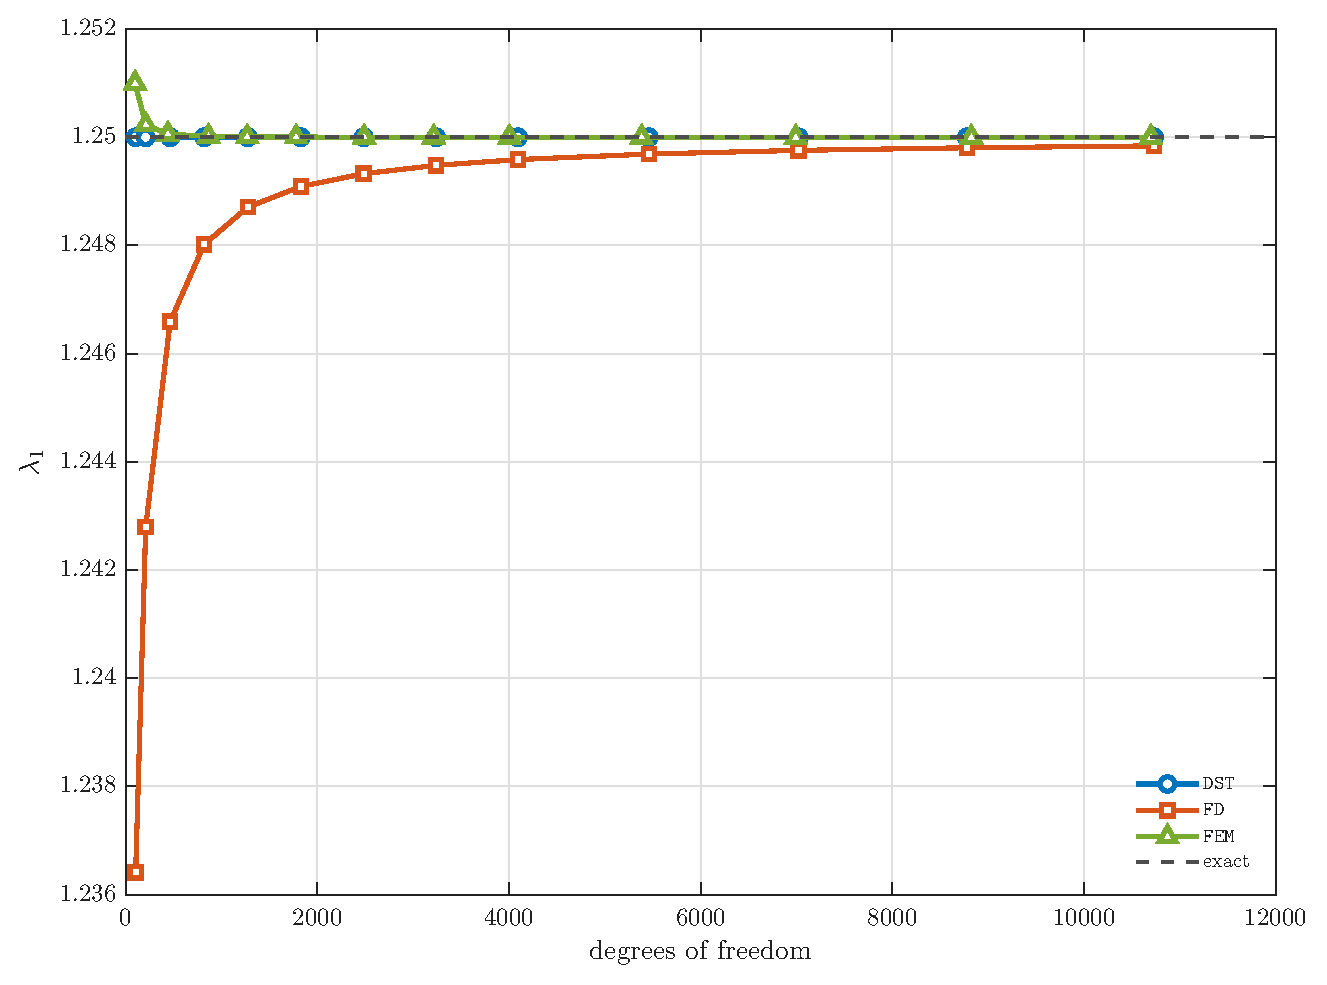
\includegraphics[width=0.45\textwidth]{rectangle_convergence_lambda1}}
  \qquad
  \subfloat[Relative error $\frac{|\lambda_1 - \lambda_1^{\text{exact}}|}{\lambda_1^{\text{exact}}}$.\label{fig:convergence_rectangle_combined_lambda1_error}]{%
    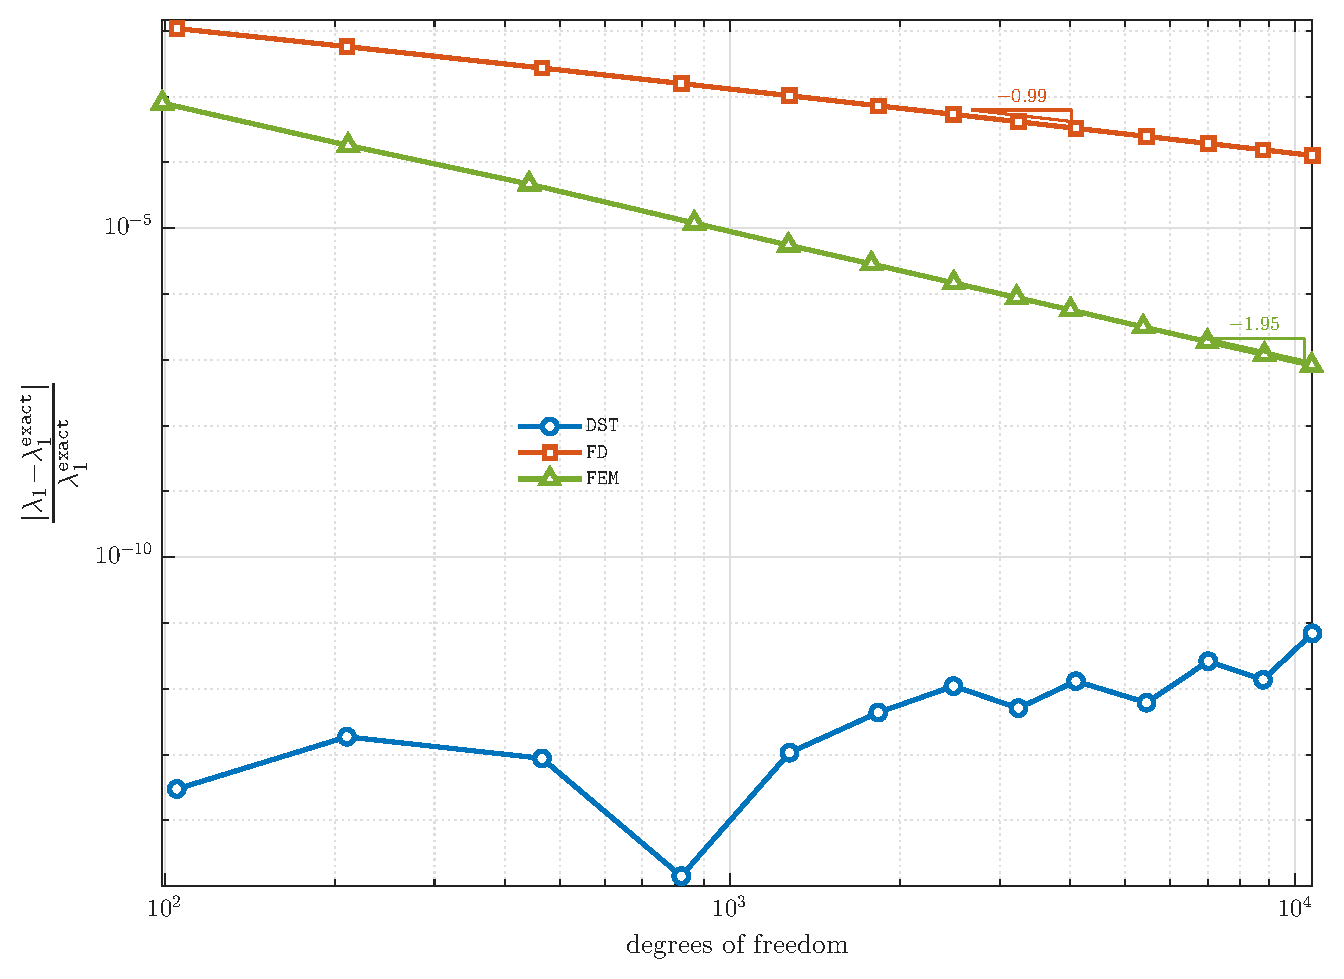
\includegraphics[width=0.45\textwidth]{rectangle_convergence_lambda1_error}}
  \\
  \subfloat[Eigenvalue $\lambda_{100}$.\label{fig:convergence_rectangle_combined_lambda100_value}]{%
    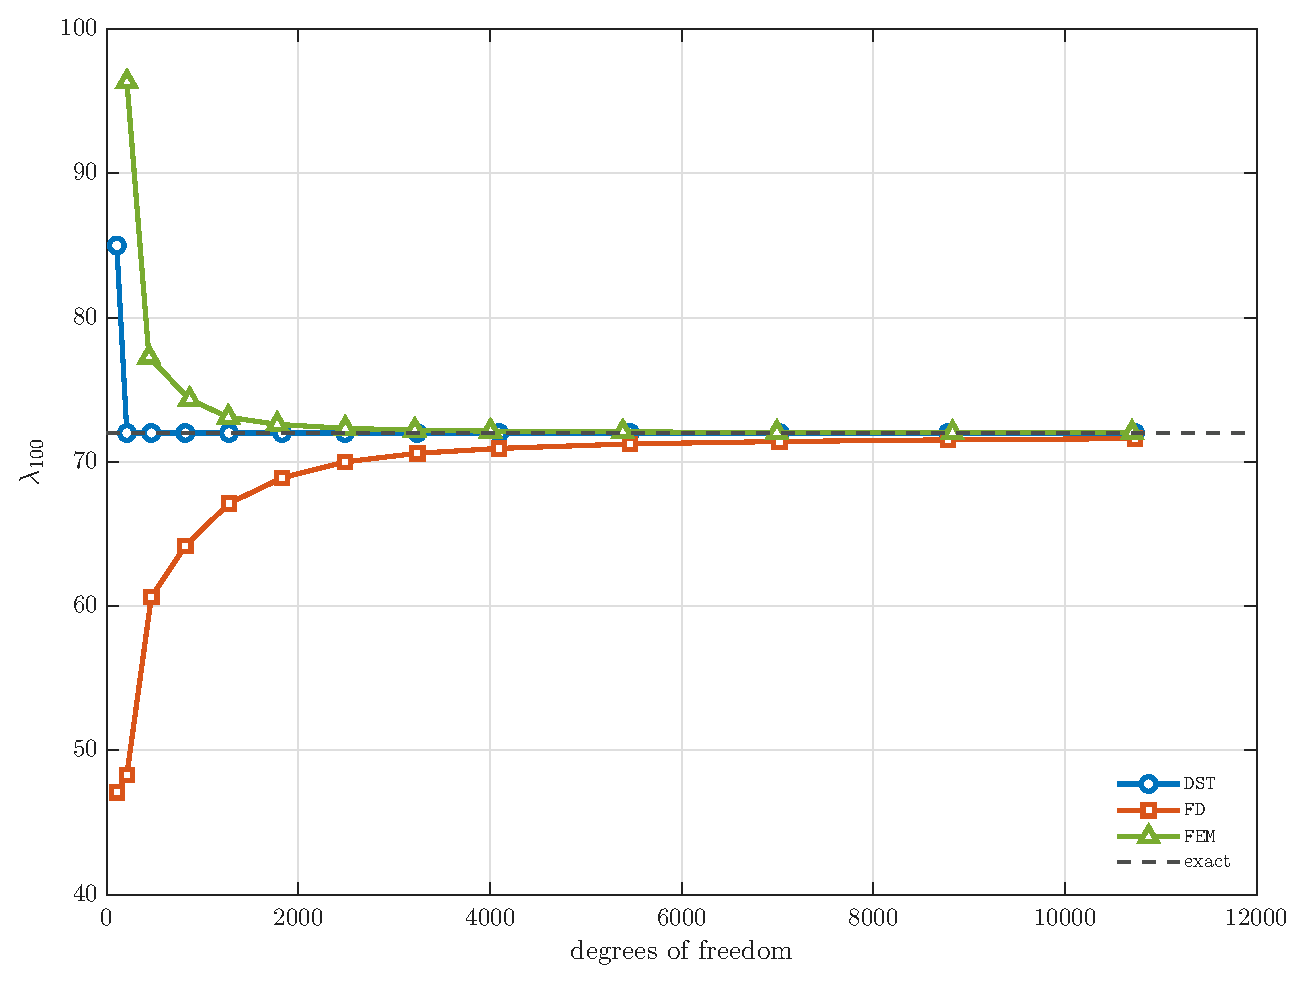
\includegraphics[width=0.45\textwidth]{rectangle_convergence_lambda100}}
  \qquad
  \subfloat[Relative error $\frac{|\lambda_{100} - \lambda_{100}^{\text{exact}}|}{\lambda_{100}^{\text{exact}}}$.\label{fig:convergence_rectangle_combined_lambda100_error}]{%
    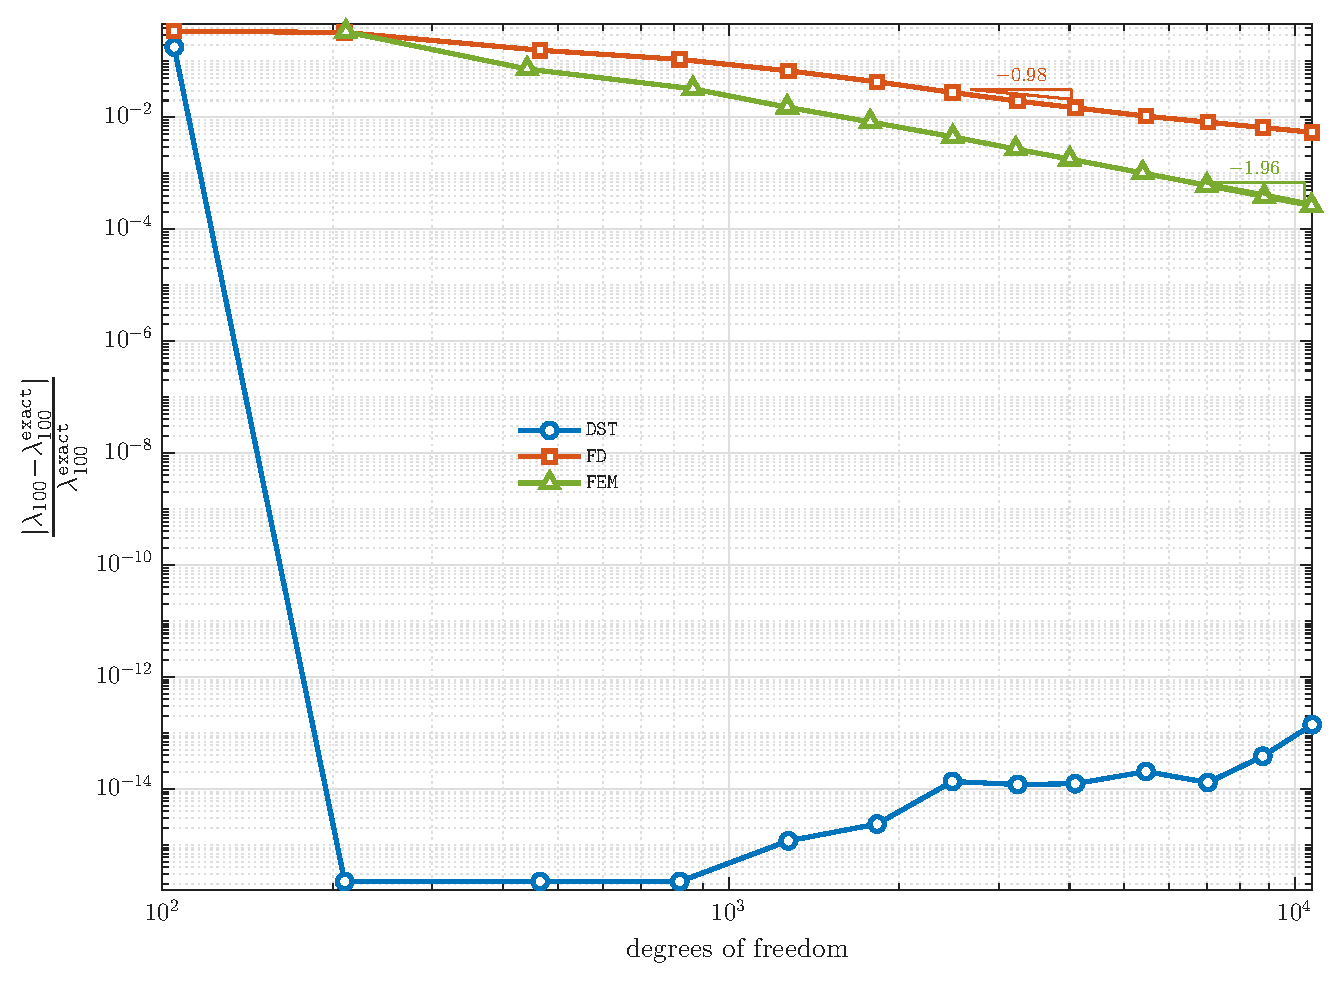
\includegraphics[width=0.45\textwidth]{rectangle_convergence_lambda100_error}}
  \\
  \subfloat[Eigenvalue $\lambda_{1000}$.\label{fig:convergence_rectangle_combined_lambda1000_value}]{%
    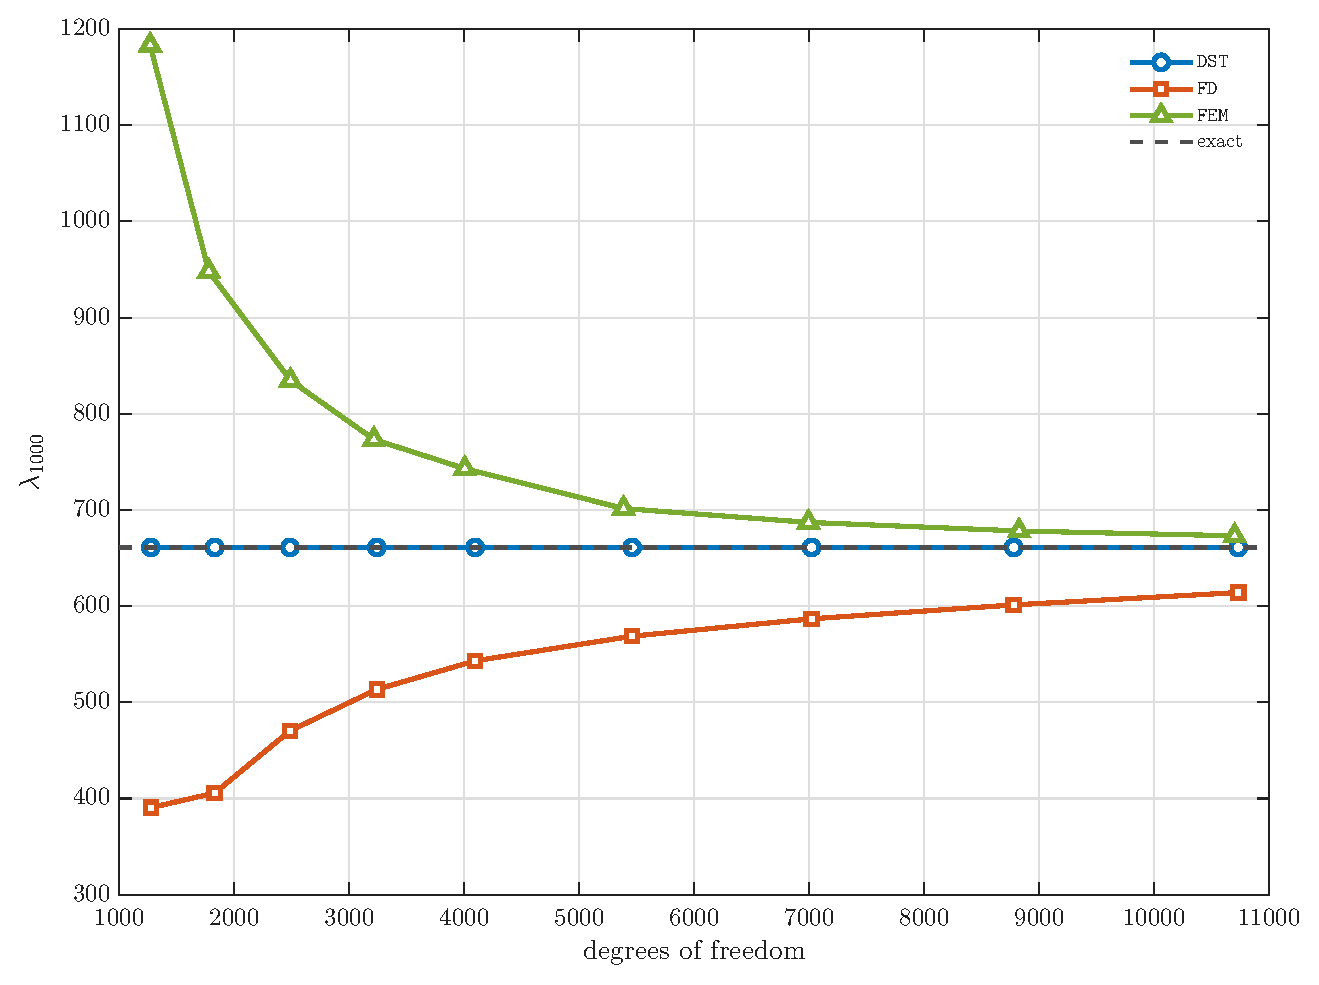
\includegraphics[width=0.45\textwidth]{rectangle_convergence_lambda1000}}
  \qquad
  \subfloat[Relative error $\frac{|\lambda_{1000} - \lambda_{1000}^{\text{exact}}|}{\lambda_{1000}^{\text{exact}}}$.\label{fig:convergence_rectangle_combined_lambda1000_error}]{%
    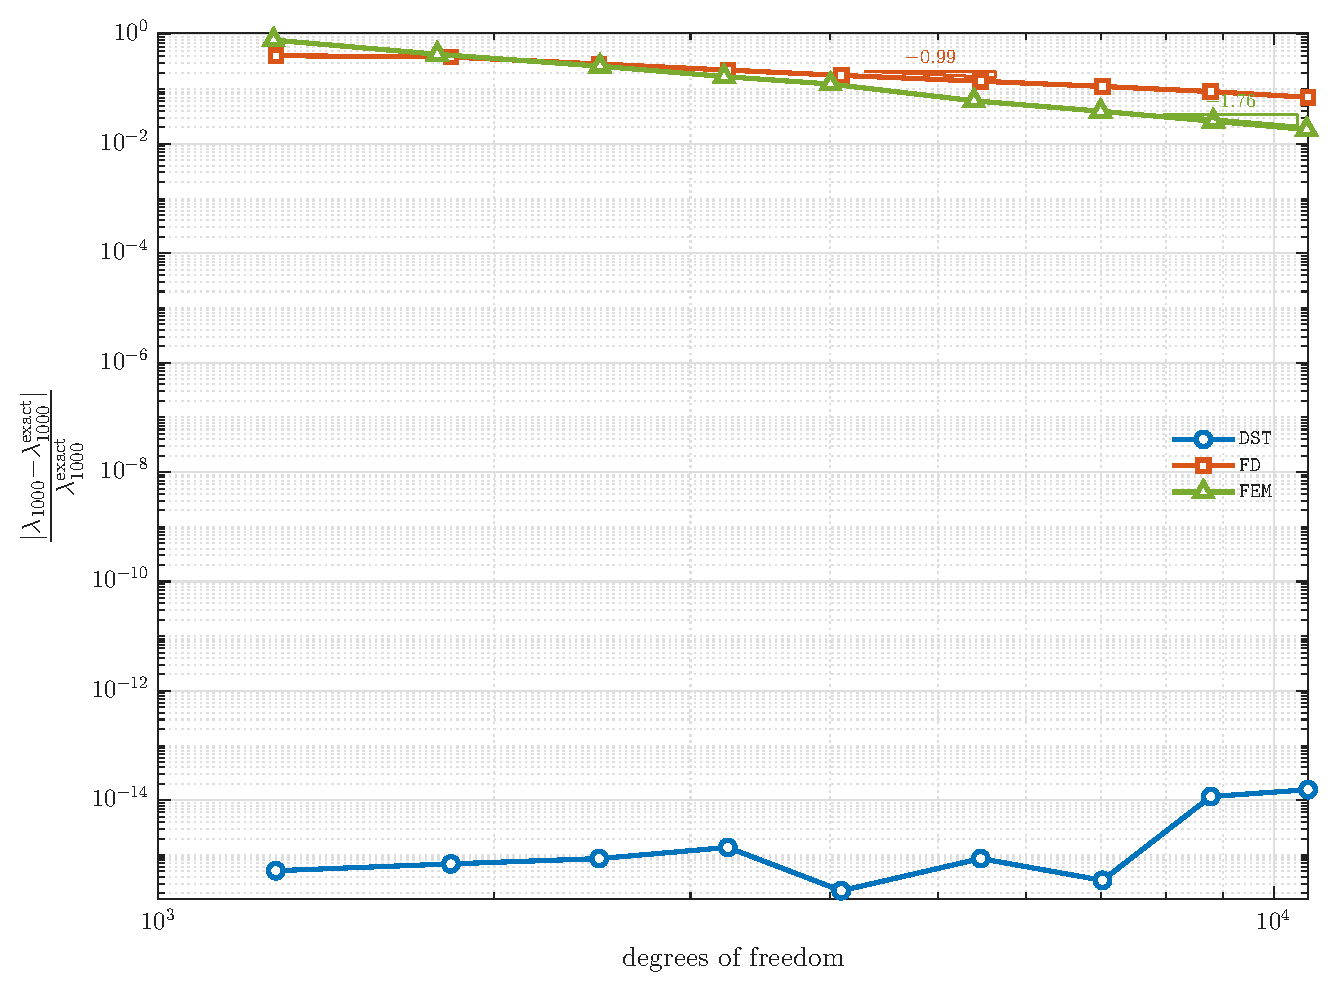
\includegraphics[width=0.45\textwidth]{rectangle_convergence_lambda1000_error}}
  \caption{Eigenvalues $\lambda_1$, $\lambda_{100}$ and $\lambda_{1000}$ of Laplace operator, zero Dirichlet boundary conditions, rectangular domain \texttt{rectangle}. Eigenvalues computed by each discretisation \texttt{DST}, \texttt{FD} and \texttt{FEM} with varying degrees of freedom; compared with the analytic/exact eigenvalues $\lambda_k^{\text{exact}}$. Resolutions carrying fewer degrees of freedom than the index of the eigenvalue cannot supply it and are left out.}
  \label{fig:convergence_rectangle}
\end{figure}
